% Từ thư mục gốc: xelatex -halt-on-error -output-directory docs docs/pfi_vton_paper_vi.tex
% Chạy hai lần để cập nhật trích dẫn. Cần XeLaTeX và phông Noto Serif/Sans.
\documentclass[11pt,a4paper]{article}
\usepackage{fontspec}
\setmainfont{Noto Serif}
\setsansfont{Noto Sans}
\usepackage{amsmath,amssymb,booktabs,graphicx,geometry,hyperref}
\geometry{margin=2.3cm}
\graphicspath{{docs/assets/}{assets/}}
\hypersetup{colorlinks=true,linkcolor=blue,citecolor=blue,urlcolor=blue}
\newcommand{\Enc}{\mathcal{E}}
\newcommand{\Dec}{\mathcal{D}}
\newcommand{\Loss}{\mathcal{L}}
\renewcommand{\refname}{Tài liệu tham khảo}
\title{PFI-VTON: Thử đồ ảo bằng Patch Forcing\\và chương trình thời gian học trang phục}
% Bổ sung tác giả, cơ quan và email theo mẫu của tạp chí trước khi nộp.
\author{}
\date{28 tháng 9 năm 2026}

\begin{document}
\maketitle
\begin{abstract}
Thử đồ ảo cần giữ nguyên người trong ảnh đồng thời chuyển đúng kiểu dáng, màu và họa tiết của áo tham chiếu. Chúng tôi xây dựng PFI-VTON bằng cách áp dụng Patch Forcing \cite{pf} cho vùng áo cần thay trong không gian tiềm ẩn. Hai luồng token người và áo dùng chung DiT tiền huấn luyện; người đọc đặc trưng áo qua attention một chiều, cho phép lưu khóa và giá trị áo giữa các bước suy luận. Trong huấn luyện, bốn kiểu lấy mẫu thời gian được phối hợp theo chương trình từ bố cục đến chi tiết, cùng giám sát tương ứng lấy cảm hứng từ CORAL \cite{coral}. Trên 256 cặp phát triển nội bộ VITON-HD ở \(512\times384\), checkpoint V41 bước 6000 đạt L1 vùng áo \(0{,}1857\) với dual-loop tám lần gọi DiT, so với \(0{,}1901\) của Euler tám lần gọi. Đây là so sánh sampler trên cùng checkpoint, chưa chứng minh hiệu quả riêng của chương trình thời gian hoặc ưu thế trước các mô hình VTON khác. Thí nghiệm ở \(1024\times768\) còn thiếu đánh giá trên tập test chính thức; một checkpoint V46 huấn luyện với cặp người--áo sai đã bị loại khỏi phân tích chất lượng.
\end{abstract}
\noindent\textbf{Từ khóa:} thử đồ ảo; Patch Forcing; flow matching; thời gian theo patch; điều kiện trang phục; suy luận ít bước.

\section{Giới thiệu}
Trong thử đồ ảo từ ảnh, đầu vào là ảnh người đã che vùng áo và ảnh sản phẩm của chiếc áo muốn mặc thử. Đầu ra cần vừa đúng người, đúng tư thế, vừa giữ đặc trưng nhận diện của áo. VITON-HD \cite{vitonhd} cung cấp ảnh gốc \(1024\times768\), nơi sai lệch ở họa tiết và đường biên dễ thấy hơn ở ảnh nhỏ. Chúng tôi nghiên cứu cách đưa áo vào DiT và cách chọn thời gian huấn luyện khi ngân sách suy luận chỉ khoảng tám lần gọi mạng.

Patch Forcing (PF) cho mỗi patch một thời gian nhiễu và dùng ước lượng độ khó để phân bổ bước lấy mẫu \cite{pf}. Điều này hợp với VTON vì nền và nhiều phần của người đã có sẵn, còn vùng áo cần tạo mới. Tuy nhiên, nếu chỉ huấn luyện trên các patch gần sạch, model có thể dựa vào chính ảnh đích thay vì học đọc áo tham chiếu. Đến khi suy luận từ nhiễu, lối tắt đó biến mất. Nếu chỉ huấn luyện với nhiễu cao, chữ nhỏ và vân vải có thể bị bỏ sót. Vì vậy, phân phối thời gian là một phần của bài toán học điều kiện áo.

Đóng góp của bản triển khai là: biểu diễn VTON thành PF inpainting; dùng chung PFT-XL/2 cho hai luồng người--áo với attention một chiều và cache áo chính xác; kết hợp bốn nhánh thời gian cùng phân tích sự khác nhau giữa trần LTG và thời gian patch thực nhận. Chúng tôi dùng DINOv3 \cite{dinov3} để tạo correspondence theo tinh thần CORAL \cite{coral}, chứ không nhận PF, DINOv3 hay correspondence distillation là phát minh của mình. Lợi ích nhân quả của từng thành phần còn cần ablation riêng.

\section{Công trình liên quan}
\textbf{Thử đồ ảo dựa trên mô hình sinh.} TryOnDiffusion \cite{tryon} kết nối các đặc trưng người và áo bằng kiến trúc hai UNet; StableVITON \cite{stableviton} học tương ứng ngữ nghĩa trong latent diffusion; CatVTON \cite{catvton} ghép không gian ảnh đầu vào để đơn giản hóa điều kiện. FitDiT \cite{fitdit} tập trung vào chi tiết áo và đặc trưng độ phân giải cao. PFI-VTON khác về cách dùng thời gian theo patch và luồng áo dùng chung block với người. Khác biệt thiết kế chưa phải bằng chứng cho chất lượng vượt các phương pháp trên, vì chưa có benchmark cùng điều kiện.

\textbf{Thời gian theo patch và tương ứng người--áo.} Flow matching \cite{flowmatching} học trường vận tốc dọc đường đi từ nhiễu tới dữ liệu. Patch Forcing \cite{pf} cho phép các patch có thời gian khác nhau và dùng độ bất định để phân bổ bước lấy mẫu; chúng tôi kế thừa ý tưởng đó cho vùng áo cần thay. CORAL \cite{coral} dùng tương ứng ngoại sinh để giám sát attention người--áo. Bản triển khai này tạo cặp ứng viên bằng đặc trưng DINOv3 đóng băng \cite{dinov3}, lọc độ tin cậy và chỉ giám sát một số head. Loss và topology attention cụ thể được xác định bằng mã dự án, không đồng nhất với toàn bộ CORAL gốc.

\section{Phương pháp}
\subsection{Định nghĩa bài toán và kiến trúc tổng thể}
Ký hiệu \(I\) là ảnh đích của người đang mặc áo \(G\), \(A\) là ảnh người đã xóa thông tin áo, \(P\) là DensePose, \(M\) là mặt nạ vùng cần sửa và \(M_G\) là mặt nạ sản phẩm áo. Ảnh đích \(I\) chỉ có khi huấn luyện hoặc đánh giá. Để supervision paired có nghĩa, áo trong \(I\) phải chính là \(G\). VAE đóng băng có encoder \(\Enc\) và decoder \(\Dec\). Với ảnh \(H\times W\), latent có \(h=H/8,\;w=W/8\). Patch latent \(2\times2\) tạo \(N=hw/4=HW/256\) token mỗi luồng: \(768\) ở \(512\times384\), \(3072\) ở \(1024\times768\).

Hình~\ref{fig:architecture} tóm tắt hai luồng xử lý và phần giám sát chỉ có khi huấn luyện. Phần tiếp theo mô tả đầu vào, attention, lịch thời gian và hàm mất mát đúng theo triển khai hiện tại.

\begin{figure}[htbp]
\centering
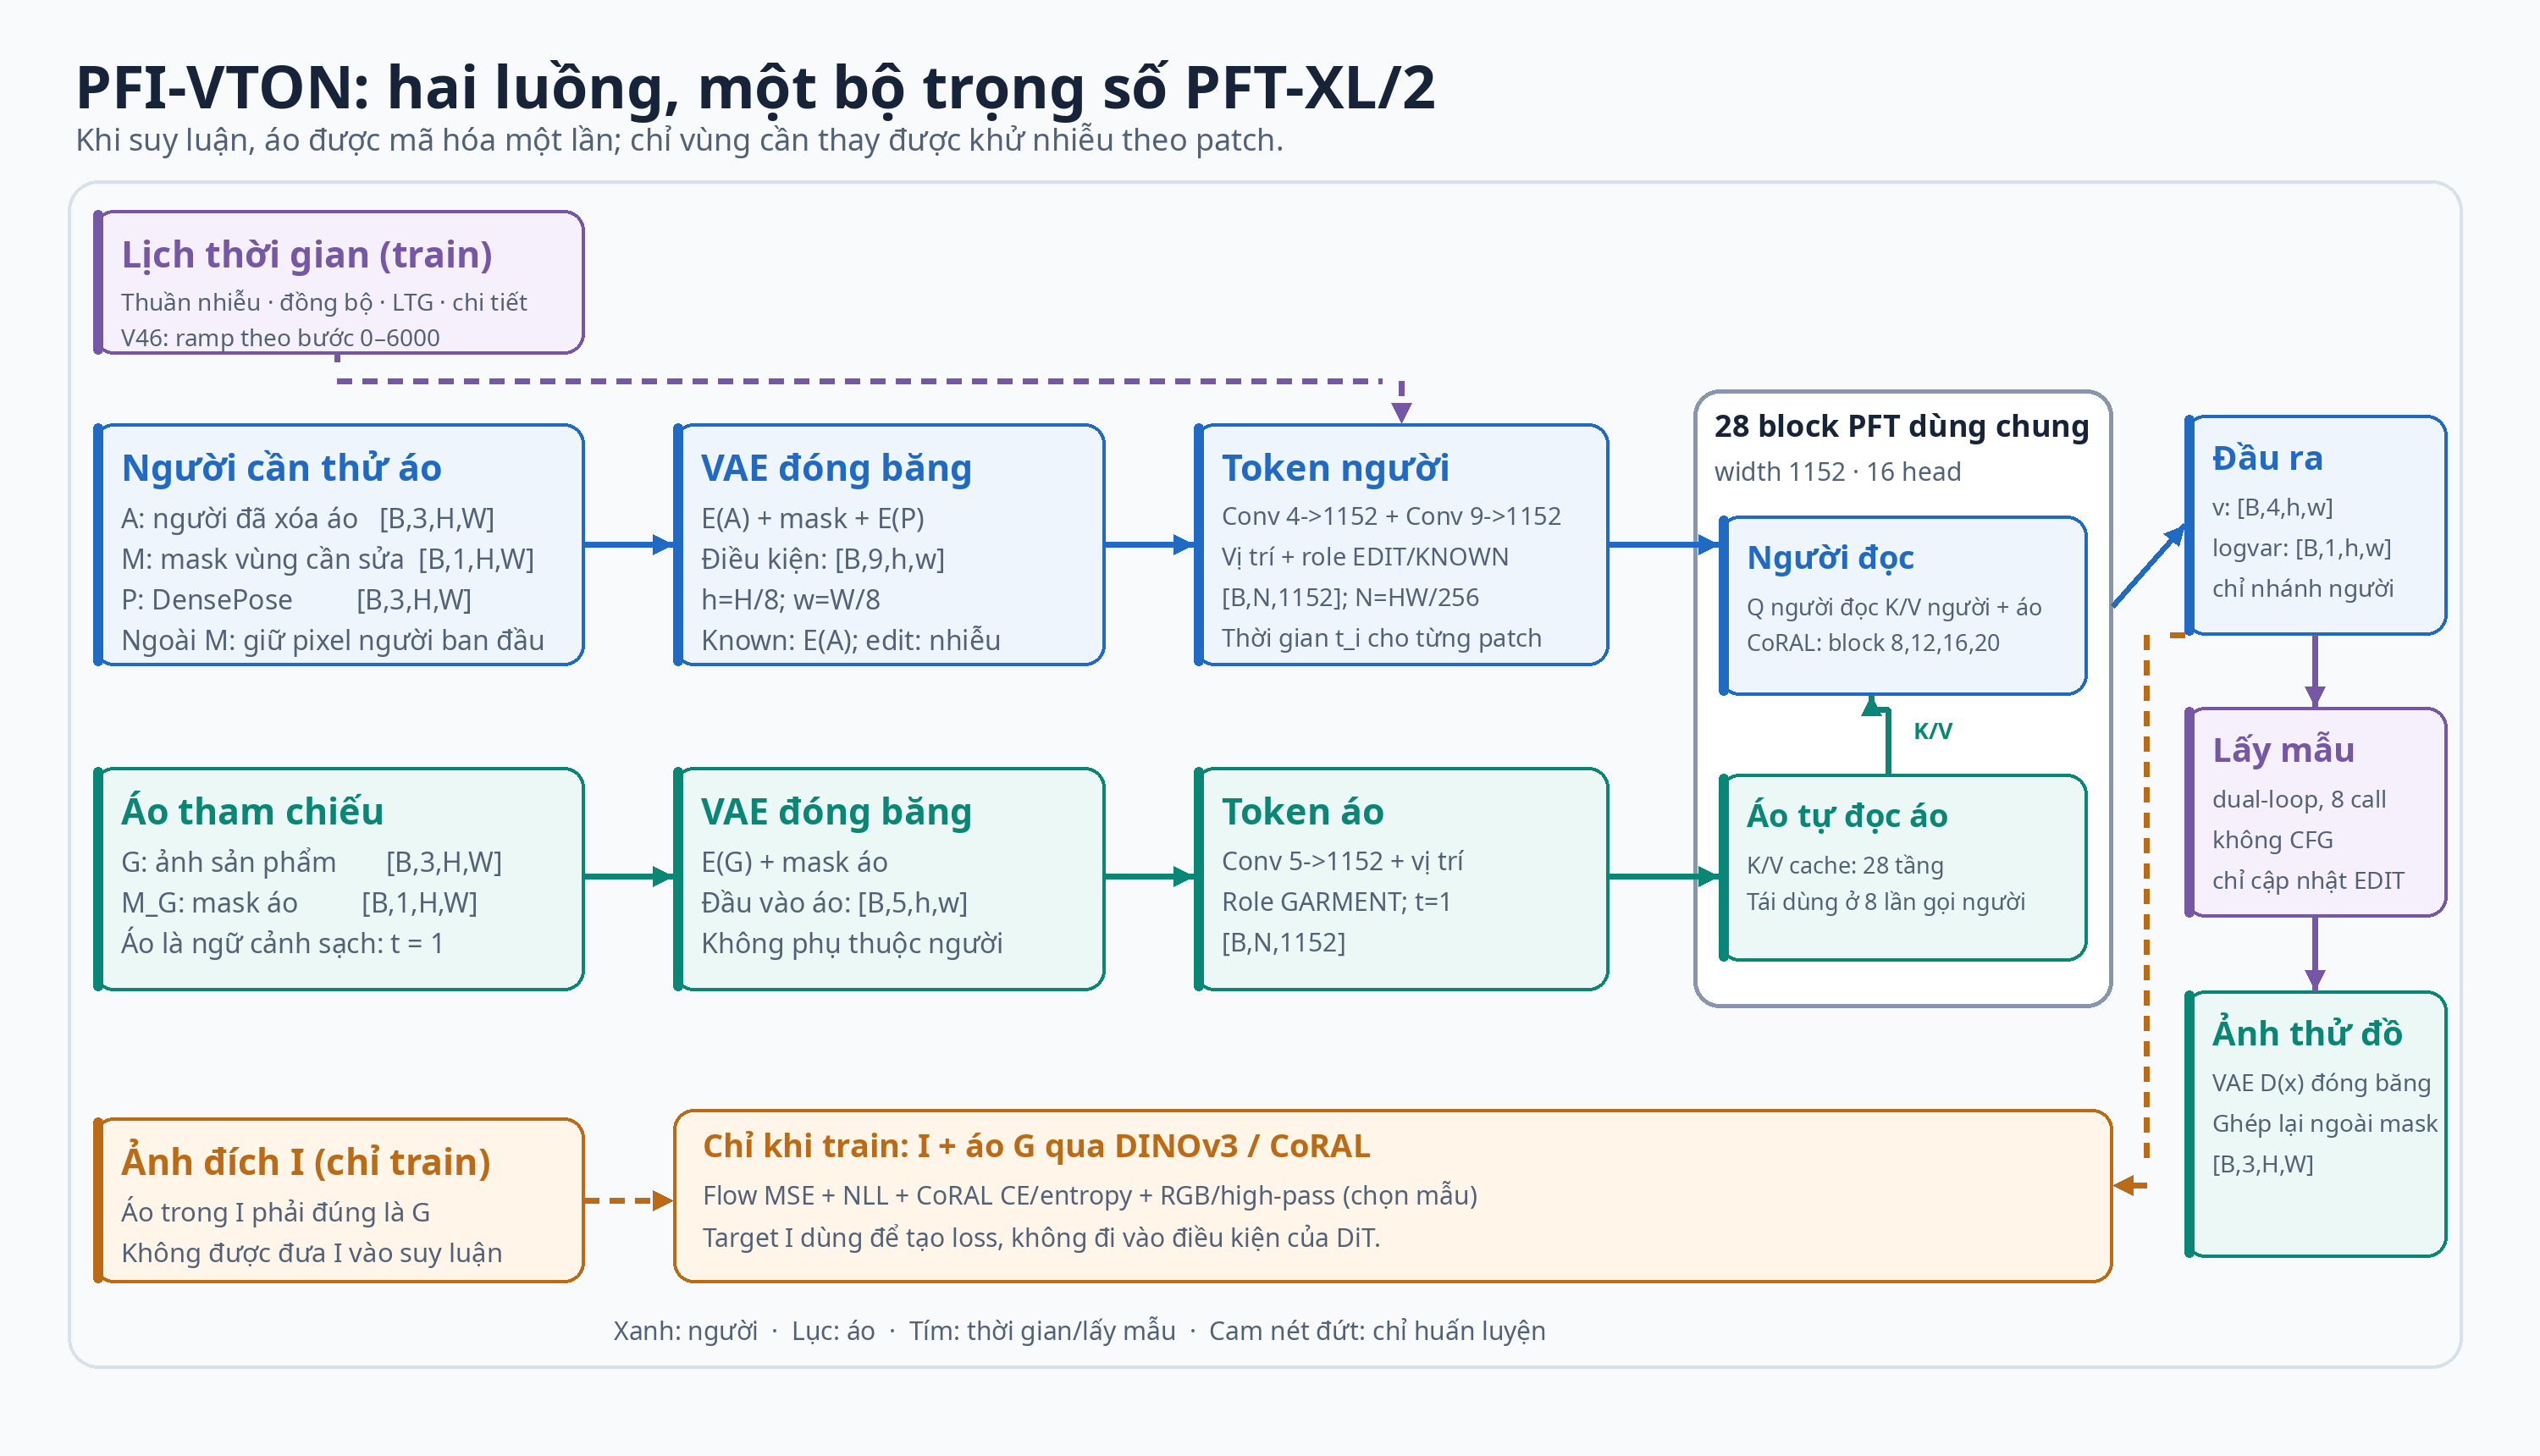
\includegraphics[width=\linewidth]{pfi-vton-architecture.png}
\caption{Kiến trúc được đối chiếu với mã model, trainer và sampler của dự án. Màu xanh là người, xanh lục là áo, tím là thời gian/lấy mẫu; cam chỉ hoạt động khi train. Tám lần gọi chỉ tính nhánh người khi không dùng CFG, chưa gồm VAE và lần mã hóa áo.}
\label{fig:architecture}
\end{figure}

\subsection{Điều kiện và kích thước}
Mặt nạ \(M\) được mở rộng để xóa mép áo cũ. Điều kiện người gồm latent agnostic bốn kênh, mask một kênh và latent DensePose bốn kênh:
\begin{equation}
c_p=[\Enc(A\odot(1-M^+)),M_\downarrow,\Enc(P)]
\in\mathbb R^{B\times9\times h\times w},\qquad
c_g=[\Enc(G),(M_G)_\downarrow]\in\mathbb R^{B\times5\times h\times w}.
\label{eq:inputs}
\end{equation}
\(M^+\) là mask sau mở rộng. Một token người là EDIT nếu patch latent giao mask; còn lại là KNOWN. Code dùng max-pooling để không đánh rơi viền áo mỏng. Pixel ngoài mask được lấy lại từ người ban đầu ở đầu ra.

\begin{center}
\begin{tabular}{lcc}
\toprule
Đại lượng mỗi luồng & \(512\times384\) & \(1024\times768\)\\
\midrule
RGB người/áo & \([B,3,512,384]\) & \([B,3,1024,768]\)\\
Latent VAE & \([B,4,64,48]\) & \([B,4,128,96]\)\\
Điều kiện người / áo & \(9/5\) kênh & \(9/5\) kênh\\
Lưới token & \(32\times24=768\) & \(64\times48=3072\)\\
Hidden mỗi luồng & \([B,768,1152]\) & \([B,3072,1152]\)\\
Đầu ra DiT & \([B,5,64,48]\) & \([B,5,128,96]\)\\
\bottomrule
\end{tabular}
\end{center}

PFT-XL/2 gốc cung cấp patch embed latent bốn kênh, 28 block rộng 1152, 16 attention head, thời gian theo token, adaLN và đầu ra năm kênh gồm vận tốc bốn kênh cùng log-phương sai một kênh \cite{pf}. PFI-VTON \emph{không giữ nguyên forward gốc}: nó thêm Conv người \(9\to1152\), Conv áo \(5\to1152\), hai bảng embedding vai trò EDIT/KNOWN/GARMENT, hai luồng attention và bảng vị trí chữ nhật. Hai Conv và hai bảng role mới có tổng cộng \(73\,728\) tham số; backbone vẫn được fine-tune. Ở \(1024\times768\), bảng vị trí gồm \(3072\times1152=3\,538\,944\) phần tử và được phép học trong V46. Bảng này được khởi tạo từ vị trí PFT gốc bằng nội suy; khi nạp checkpoint cùng độ phân giải, vị trí đã học được giữ lại.

\subsection{Attention một chiều và cache áo}
Ở tầng \(\ell\), áo chỉ tự attention; người đọc cả token người lẫn áo:
\begin{align}
A_\ell^g&=\operatorname{softmax}\left(Q_\ell^g(K_\ell^g)^\top/\sqrt{72}\right),\\
A_\ell^p&=\operatorname{softmax}\left(Q_\ell^p[K_\ell^p;K_\ell^g]^\top/\sqrt{72}\right).
\label{eq:attention}
\end{align}
Mỗi head có \(1152/16=72\) chiều; phép nối \([K^p;K^g]\) có \(2N\) key. Cùng một bộ trọng số block chạy cho hai luồng, nhưng áo không nhận thông tin từ người. Do đó \((K_\ell^g,V_\ell^g)\) của 28 tầng không đổi giữa các lần gọi DiT và có thể cache một lần cho mỗi ảnh áo. Đây là tính chất chính xác của hướng attention trong code, không phải mạng áo thứ hai hay cache xấp xỉ. CFG khác 1 cần thêm cache áo rỗng.

\subsection{Teacher tương ứng người--áo}
Ở các block chỉ số \(8,12,16,20\), bốn head đầu trả thêm attention từ người sang áo. DINOv3-S/16 đóng băng mã hóa \(I\) và \(G\), tìm patch áo tương tự nhất với mỗi patch người và lọc bằng độ tương đồng cùng nhất quán chu trình. Với query tin cậy \(i\), vị trí match \(j^*(i)\), đích Gaussian và attention được giám sát là:
\begin{equation}
T_{ij}\propto\mathbf1_{j\in G_{\rm valid}}
\exp\left(-\|r_j-r_{j^*(i)}\|^2/(2\sigma^2)\right),\qquad
a_{ij}^{\ell q}=\operatorname{softmax}_{j\in G}
\left(Q^p_{\ell q,i}(K^g_{\ell q,j})^\top/\sqrt{72}\right).
\label{eq:coral}
\end{equation}
\(T\) được chuẩn hóa trên patch áo hợp lệ. Loss cross-entropy của từng head với \(T\) được trung bình trên các query tin cậy, bốn head và bốn block, rồi chia cho \(\log N\); entropy của \(a\) cũng được phạt. V46 dùng \(\sigma=0{,}02\) theo tọa độ chuẩn hóa. \emph{\(a\) chỉ chuẩn hóa trên key áo}; attention thực trong \eqref{eq:attention} chuẩn hóa chung trên key người và áo. Vì vậy \texttt{coral\_local\_mass} cho biết vị trí được chọn \emph{khi đọc áo}, chưa chứng minh model dành nhiều attention tuyệt đối cho áo. DINOv3 và loss này không chạy lúc suy luận.

\subsection{Huấn luyện theo thời gian patch}
\subsubsection{Flow matching trên vùng cần sửa}
Với ảnh đích \(I\), đặt \(z_1=\Enc(I)\), \(\epsilon\sim\mathcal N(0,\mathbf I)\) và \(k=\Enc(A\odot(1-M^+))\). Thời gian \(t_i\) của token EDIT được trải tới bốn ô latent thuộc patch. Ở ô latent \(p\):
\begin{equation}
z_{t,p}=
\begin{cases}
t_pz_{1,p}+(1-t_p)\epsilon_p,&p\in\mathrm{EDIT},\\
k_p,&p\in\mathrm{KNOWN},
\end{cases}
\qquad u_p=z_{1,p}-\epsilon_p\quad(p\in\mathrm{EDIT}).
\label{eq:flowpath}
\end{equation}
Đây là đường nội suy tuyến tính của flow matching \cite{flowmatching}: \(t=0\) là nhiễu, \(t=1\) là dữ liệu. KNOWN luôn có \(t=1\) nhưng chứa \(k\), \emph{không phải} latent ảnh đích. Token áo cũng luôn sạch và có \(t=1\). Cách này tránh đưa \(I\) vào điều kiện người trong lúc train.

\subsubsection{Bốn nhánh thời gian và hai lịch khác nhau}
Với mỗi ảnh ở bước cập nhật \(s\), code chọn một trong bốn nhánh:
\begin{equation}
q_s=\pi_0(s)q_{\rm noise}+\pi_S(s)q_{\rm sync}
+\pi_D(s)q_{\rm detail}+\pi_L(s)q_{\rm LTG},\quad
\pi_L(s)=1-\pi_0(s)-\pi_S(s)-\pi_D(s).
\label{eq:mixture}
\end{equation}
Nhánh noise đặt mọi \(t_i=0\); sync cho các patch EDIT cùng một thời gian; LTG cho thời gian khác nhau theo patch; detail ưu tiên trạng thái gần sạch. Ở \(t=0\), vùng EDIT không chứa latent ảnh đích, nên model phải dựa nhiều hơn vào áo, tư thế và ngữ cảnh người. Đây là động cơ, chưa phải bằng chứng nhân quả rằng riêng nhánh noise cải thiện chất lượng.

Trong LTG, \(\bar t\) là \emph{cận trên} chứ không phải trung bình thời gian patch. Với \(\eta_i\sim\mathcal N(0,1)\), code lấy
\begin{equation}
\widetilde t_i=\bar t-|\eta_i|\min(\bar t/2,\sigma_k).
\label{eq:lag}
\end{equation}
Giá trị âm được thay bằng mẫu đều trong \([0,\bar t]\). Detail ở V41 trở đi dùng \(\sigma_D=0{,}05\); LTG thường dùng \(\sigma_L=0{,}6\). Cận độ lệch chỉ áp vào detail nên tạo thêm ví dụ thật sự gần sạch. Ở \(1024\times768\), V46 dùng phép dịch
\begin{equation}
S_a(t)=\frac{t}{t+a(1-t)},\qquad a=2
\label{eq:shift}
\end{equation}
cho ba nhánh thường, còn detail giữ thời gian chưa dịch. \(a>1\) kéo thời gian về phía nhiễu.

Cần phân biệt hai lịch đã thử. V40--V42 có cổng metric: EMA của \texttt{coral\_local\_mass} phải đạt \(0{,}30\) sau ít nhất 1500 bước, hoặc cổng tự mở ở bước 6000; ramp sau đó dài 3000 bước. V46 \emph{không chờ CoRAL đạt ngưỡng}: \texttt{gate\_max\_steps=0} làm ramp bắt đầu ở cập nhật đầu và dài 6000 bước. Gọi \(\alpha_s\in[0,1]\) là tiến độ ramp, ta có
\begin{equation}
(\pi_0,\pi_S,\pi_D,\pi_L)_s
=(1-\alpha_s)(0{,}35,0{,}25,0,0{,}40)
+\alpha_s(0{,}10,0{,}15,0{,}40,0{,}35),\quad
\mathrm{loc}_{\rm LTG}(s)=-1+1{,}8\alpha_s.
\label{eq:v46schedule}
\end{equation}
Lúc đầu mô hình gặp nhiều ví dụ chưa có áo trên người; về sau gặp thêm ví dụ chỉ cần sửa chi tiết. Đây là lịch theo \emph{số bước của run}, không phải cổng correspondence của V40. Khi khởi tạo từ snapshot chỉ có trọng số, optimizer và bộ đếm của run mới bắt đầu từ 0.

\subsubsection{Hàm mất mát ở V46}
Gọi \(m_p\) là mask EDIT ở latent, \(C_p\) là mask parse áo đã đưa về latent, \(v_{\theta,p}\) là vận tốc và \(s_{\theta,p}\) là log-phương sai. Ký hiệu \(\langle\cdot\rangle_c\) là trung bình bốn kênh latent. Phần flow và uncertainty đúng với chuẩn hóa trong code là
\begin{align}
w_p&=m_p(1+C_p),&
\Loss_{\rm flow}
&=\frac{\sum_p w_p\langle(v_{\theta,p}-u_p)^2\rangle_c}
{\sum_p w_p},\label{eq:flowloss}\\
\Loss_{\rm nll}
&=\frac{\sum_p m_p\,\tfrac12
\left(s_{\theta,p}+e^{-s_{\theta,p}}
\langle(u_p-\operatorname{sg}(v_{\theta,p}))^2\rangle_c\right)}
{\sum_p m_p}.\label{eq:nll}
\end{align}
\(\operatorname{sg}\) dừng gradient để uncertainty head học độ khó mà không kéo vận tốc qua loss này. Với ảnh đủ điều kiện (\(\bar t_{\rm EDIT}\geq0{,}65\), không dropout áo, được chọn xác suất \(0{,}5\), tối đa một ảnh mỗi microbatch), điểm cuối dự đoán là
\begin{equation}
\widehat z_{1,p}=z_{t,p}+(1-t_p)v_{\theta,p},\qquad
\widehat I=\Dec(\widehat z_1).
\label{eq:endpoint}
\end{equation}
Decoder VAE đóng băng tham số, nhưng gradient loss ảnh vẫn đi \emph{qua} decoder về DiT. V46 tính L1 RGB và L1 cao tần trên ảnh được giải mã đầy đủ; vùng chấm điểm là giao giữa mask áo và EDIT. Trọng số tăng ở vùng khác màu nền áo được suy từ ảnh đích chỉ để tính loss, không phải nhãn ký tự hay điều kiện suy luận.

Nếu \(\Loss_{\rm CE},\Loss_{\rm ent}\) là loss correspondence và entropy, \(\gamma\in\{0,1\}\) cho biết ảnh đã được chọn cho loss giải mã, mục tiêu là
\begin{equation}
\Loss=\Loss_{\rm flow}+0{,}01\Loss_{\rm nll}
+0{,}10\Loss_{\rm CE}+0{,}01\Loss_{\rm ent}
+\gamma(0{,}5\Loss_{\rm RGB}+2{,}0\Loss_{\rm HP}).
\label{eq:total}
\end{equation}
V46 đặt \texttt{decoded\_follow\_curriculum=false}: không nhân thêm loss giải mã với tiến độ ramp. Tuy nhiên, điều kiện \(t\geq0{,}65\) làm loss này xuất hiện thường hơn khi lịch có nhiều thời gian muộn.

\subsection{Suy luận trong ngân sách tám lần gọi DiT}
Suy luận bắt đầu bằng nhiễu Gaussian trong EDIT và latent agnostic sạch ngoài mask. Luồng áo mã hóa một lần thành 28 cặp K/V. Ở mỗi vòng ngoài dual-loop, \(\exp(s_\theta)\) được gộp theo patch để ước lượng độ bất định; tại phân vị \(p=0{,}7\), khoảng 30\% token EDIT khó đi thành hai bước nhỏ, còn token dễ đi trọn bước. Bốn vòng ngoài nhân hai lần đánh giá tạo tám lần gọi DiT nhánh người khi CFG bằng 1. \emph{Mỗi lần gọi vẫn xử lý toàn bộ chuỗi token người}; 30\% patch khó không có nghĩa chỉ tốn 30\% phép tính Transformer. CFG khác 1 có thể cần 16 lần gọi người và hai cache áo. Cuối cùng VAE giải mã latent; pixel người đã quan sát ngoài mask được ghép lại.

\section{Thiết lập thực nghiệm}
\subsection{Dữ liệu và ghép cặp}
Với paired training, chiếc áo trong ảnh target phải trùng ảnh áo điều kiện. Tập VITON-HD nội bộ được tách bằng stable hash seed 2026: 11\,391 cặp fit và 256 cặp dev. Dev này không phải test chính thức. File \texttt{train\_pairs.txt} trong ZIP hiện có chủ yếu chứa cặp \emph{unpaired}, phù hợp cho thử áo khác ở suy luận nhưng không thể làm target tái tạo paired. Data loader và trainer hiện kiểm tra danh tính áo, fit/dev không chồng lấn và fingerprint cặp khi resume.

\subsection{Cấu hình huấn luyện và checkpoint}
Các kết quả định lượng chính ở \(512\times384\) đến từ V41: mô hình tiếp tục từ V40 bước 5000 với optimizer và trạng thái chương trình thời gian được giữ lại, rồi đánh giá checkpoint ở bước 5500 và 6000. V41 chỉ thu hẹp độ lệch thời gian của nhánh detail; chưa có thí nghiệm đối chứng độc lập với cùng trọng số và cùng số lần cập nhật. Các pilot V43--V46 dùng ảnh \(1024\times768\), thay đổi cả cách khởi tạo và loss nên không được gộp với bảng V41 thành một đường cải thiện duy nhất. Bảng~\ref{tab:setup} ghi những thiết lập cần để đọc đúng hai nhóm kết quả.

\begin{table}[htbp]
\centering
\caption{Cấu hình liên quan đến các kết quả được báo cáo. V46 sạch là thiết lập nghiên cứu ở độ phân giải cao, chưa có benchmark test chính thức.}
\label{tab:setup}
\begin{tabular}{lcc}
\toprule
Thiết lập & V41 & V46 sạch\\
\midrule
Ảnh \(H\times W\) & \(512\times384\) & \(1024\times768\)\\
Latent \(h\times w\) & \(64\times48\) & \(128\times96\)\\
Microbatch \(\times\) tích lũy & \(4\times4\) & \(4\times4\)\\
LR đỉnh backbone & \(2\times10^{-5}\) & \(2\times10^{-5}\)\\
LR đỉnh module mới & \(10^{-4}\) & \(4\times10^{-5}\)\\
Mở mask lúc train & \(0\)--\(12\) px & \(0\)--\(24\) px\\
Loss ảnh giải mã & Không & RGB + cao tần, toàn ảnh\\
Lịch thời gian & Cổng metric V40 & Ramp 6000 bước\\
\bottomrule
\end{tabular}
\end{table}

\subsection{Giao thức đánh giá và thước đo}
Audit V41 dùng cùng 256 cặp paired dev, cùng nhiễu cho mỗi ảnh khi đổi sampler hoặc checkpoint. Euler và dual-loop được so theo số lần gọi bộ khử nhiễu nhánh người; mã hóa áo một lần và VAE chưa được tính vào ngân sách này. Các chỉ số là L1 trên vùng EDIT, vùng áo, vùng chi tiết tương phản, L1 cao tần ở vùng tương phản và SSIM vùng áo \cite{ssim}. Ảnh RGB được chuẩn hóa về \([-1,1]\). Vùng tương phản được tạo từ màu đích để kiểm toán họa tiết, không phải nhãn chữ hay metric OCR. Tám ảnh preview cố định dùng để xem lỗi trực quan; chúng không thay cho 256 cặp dev. Chưa có số liệu test chính thức, độ trễ đầu-cuối hoặc so sánh baseline VTON trong cùng giao thức.

\section{Kết quả}
\subsection{Độ bao phủ thời gian ở \(512\times384\)}
Kiểm toán đúng bộ lấy mẫu trên \(16\,384\) ví dụ, mỗi ví dụ 64 token, cho thấy sửa nhánh detail từ V40 sang V41 đổi phân phối như Bảng~\ref{tab:time}. Đây là phép đo thời gian được lấy mẫu, chưa chứng minh ảnh đẹp hơn.
\begin{table}[htbp]
\centering
\caption{Thời gian patch trong kiểm toán V40--V41.}
\label{tab:time}
\begin{tabular}{lcc}
\toprule
Chỉ số & V40 & V41\\
\midrule
Trung bình \(t\) của nhánh detail & \(0{,}5313\) & \(0{,}8250\)\\
Patch detail có \(t>0{,}8\) & \(10{,}22\%\) & \(60{,}95\%\)\\
Patch detail có \(t>0{,}9\) & \(1{,}96\%\) & \(18{,}28\%\)\\
Hỗn hợp cuối có \(t>0{,}8\) & \(5{,}61\%\) & \(26{,}14\%\)\\
Hỗn hợp cuối có \(t>0{,}9\) & \(0{,}96\%\) & \(7{,}48\%\)\\
\bottomrule
\end{tabular}
\end{table}

\subsection{Chất lượng theo sampler trên tập dev}
Bảng~\ref{tab:sampler} báo cáo các giá trị trung bình theo giao thức ở mục thiết lập thực nghiệm. L1 nhỏ hơn tốt hơn, SSIM lớn hơn tốt hơn. V41-5500 và V41-6000 không phải ablation độc lập vì checkpoint sau đã train thêm 500 bước.
\begin{table}[htbp]
\centering
\caption{Sampler nội bộ ở \(512\times384\). HP là L1 cao tần vùng tương phản trên áo.}
\label{tab:sampler}
\begin{tabular}{llrrrr}
\toprule
Checkpoint & Sampler/call & EDIT L1 & Áo L1 & HP L1 & SSIM áo\\
\midrule
V41-5500 & Euler/8 & \(0{,}1697\) & \(0{,}1948\) & \(0{,}1583\) & \(0{,}5448\)\\
V41-5500 & Dual-loop/8 & \(0{,}1655\) & \(0{,}1902\) & \(0{,}1563\) & \(0{,}5553\)\\
V41-6000 & Euler/8 & \(0{,}1678\) & \(0{,}1901\) & \(0{,}1579\) & \(0{,}5530\)\\
V41-6000 & Dual-loop/8 & \(0{,}1637\) & \(0{,}1857\) & \(0{,}1561\) & \(0{,}5632\)\\
V41-6000 & Euler/25 & \(0{,}1764\) & \(0{,}2007\) & \(0{,}1640\) & \(0{,}5304\)\\
\bottomrule
\end{tabular}
\end{table}
Ở V41-6000, dual-loop/8 giảm L1 vùng áo trung bình \(0{,}0044\), tương đương khoảng \(2{,}3\%\), so với Euler/8 cùng ngân sách. Sai số chuẩn của riêng trung bình L1 vùng áo xấp xỉ \(0{,}007\); chưa có khoảng tin cậy theo \emph{chênh lệch ghép cặp} giữa hai sampler nên không thể tuyên bố khác biệt có ý nghĩa thống kê. Euler/25 có L1 vùng áo cao hơn trong cùng audit, nhưng thêm bước không phải thí nghiệm cô lập toàn bộ nguyên nhân. Preview cho thấy màu, kiểu và vị trí đồ họa thường dễ giữ hơn ký tự; chữ như Lee và FILA vẫn có thể sai.

\subsection{Pilot \(1024\times768\) và kiểm toán lỗi dữ liệu V46}
V43--V45 là các pilot cùng kiến trúc nhưng khác khởi tạo, loss và cách giải mã. Trên tám ảnh cố định V43, ảnh sắc hơn đôi khi lại có L1 cao hơn vì họa tiết lệch vài pixel; chưa có đối sánh full-dev giữa các bản này. V46 dùng loss giải mã toàn ảnh, lịch \eqref{eq:v46schedule}, batch hiệu dụng \(4\times4=16\) và PFT-XL/2 fine-tune ở độ phân giải gốc.

Một lần tiếp tục V46 đã đọc nhầm cặp unpaired: 11\,390/11\,391 hàng fit có áo không trùng áo trong ảnh đích. Flow/RGB loss lúc ấy phạt model nếu nó làm theo áo tham chiếu sai, còn CoRAL nhận correspondence không thích hợp. Trên tám cặp đúng cố định, L1 vùng áo của checkpoint hỏng bước 3000 là \(0{,}7737\), so với khoảng \(0{,}19\) của snapshot sạch bước 1500. Đây là \emph{chẩn đoán lỗi dữ liệu}, không phải kết quả chất lượng của lịch V46. Checkpoint hỏng bị loại; run mới dùng trọng số sạch bước 1500, optimizer mới và danh sách paired được xác minh. Xem kiểm toán \path{docs/v46_resume_regression_audit_20260927.md}.

\section{Thảo luận và giới hạn}
Kết quả xác nhận mô hình có thể chạy luồng người--áo với thời gian theo patch và đo được sự thay đổi phân phối thời gian khi thu hẹp độ lệch của nhánh detail. Kết quả sampler ở cùng checkpoint gợi ý dual-loop có ích trong ngân sách tám call, nhưng thí nghiệm hiện tại không tách riêng tác dụng của lịch thời gian, CoRAL hay khởi tạo pretrained. V41-6000 và V41-5500 khác số bước train, còn các pilot \(1024\times768\) thay đổi nhiều thành phần cùng lúc.

Mục tiêu dưới mười bước hiện chỉ tính call DiT nhánh người khi không dùng CFG, chưa có đo độ trễ đầu-cuối, VRAM suy luận hay đối sánh công bằng với VTON khác. Từ \(512\times384\) lên \(1024\times768\), số token mỗi luồng tăng bốn lần và số cặp query--key tăng mười sáu lần. SDPA không nhất thiết lưu toàn bộ ma trận attention, nhưng DINOv3 và các map CoRAL khi train vẫn tốn bộ nhớ. Cache áo tránh tính lại áo, không xóa chi phí attention người.

L1/SSIM paired không đo được chữ có đúng từ hay logo đúng thương hiệu. Cần test chính thức, LPIPS \cite{lpips}, OCR có nhãn kiểm tra, phép can thiệp áo đúng/áo tráo/áo rỗng cùng người và seed; đồng thời ablation từ cùng checkpoint cho pure noise, detail, CoRAL và sampler. Dữ liệu dev là paired nên chưa chứng minh khả năng tổng quát sang cặp người--áo chưa từng xuất hiện cùng nhau. Cũng cần báo khoảng tin cậy cho chênh lệch metric ghép cặp và đo latency gồm VAE cùng mã hóa áo. Chỉ khi ấy mới có thể kết luận về ưu thế VTON dưới mười bước.

\section{Kết luận}
PFI-VTON diễn đạt thử áo thành PF inpainting trong latent: vùng người đã biết được giữ lại, vùng sửa có thời gian riêng theo patch, áo tham chiếu là luồng sạch dùng chung DiT. Hướng attention từ người sang áo cho phép cache K/V đúng theo forward. Bốn nhánh thời gian được thiết kế để vừa học đọc áo từ nhiễu, vừa học phần chi tiết gần sạch. Trên 256 cặp dev ở \(512\times384\), dual-loop tám call có L1/SSIM trung bình nhỉnh hơn Euler tám call; độ tin cậy thống kê, bảo toàn chữ/logo và tổng quát hóa ở \(1024\times768\) còn phải kiểm chứng. Kiểm toán V46 nhấn mạnh rằng cặp người--áo phải đúng trước khi diễn giải loss hoặc preview.

\section*{Tính tái lập và nguồn kết quả nội bộ}
Kiến trúc: \path{vton_ext/pfi_model.py}; đầu vào/lấy mẫu: \path{vton_ext/pfi_sample.py}; thời gian/loss: \path{vton_ext/pfi_train.py}; teacher: \path{vton_ext/coral.py}. Audit V40--V42: \path{docs/pfi_vton_method.md}, \path{docs/vton_v41_detail_pilot.md} và \path{docs/assets}. Sơ đồ được tạo lại bằng \path{scripts/render_pfi_vton_architecture.py}. Đây là kiểm toán của dự án, không thay benchmark độc lập.

\begin{thebibliography}{99}
\bibitem{pf} J. Schusterbauer, M. Gui, Y. Li, P. Ma, F. Krause, B. Ommer. \emph{Denoising, Fast and Slow: Difficulty-Aware Adaptive Sampling for Image Generation}. CVPR, 2026. \url{https://openaccess.thecvf.com/content/CVPR2026/html/Schusterbauer_Denoising_Fast_and_Slow_Difficulty-Aware_Adaptive_Sampling_for_Image_Generation_CVPR_2026_paper.html}.
\bibitem{flowmatching} Y. Lipman, R. T. Q. Chen, H. Ben-Hamu, M. Nickel, M. Le. \emph{Flow Matching for Generative Modeling}. ICLR, 2023. \url{https://openreview.net/forum?id=PqvMRDCJT9t}.
\bibitem{vitonhd} S. Choi, S. Park, M. Lee, J. Choo. \emph{VITON-HD: High-Resolution Virtual Try-On via Misalignment-Aware Normalization}. CVPR, 2021. \url{https://openaccess.thecvf.com/content/CVPR2021/html/Choi_VITON-HD_High-Resolution_Virtual_Try-On_via_Misalignment-Aware_Normalization_CVPR_2021_paper.html}.
\bibitem{tryon} L. Zhu, D. Yang, T. Zhu, F. Reda, W. Chan, C. Saharia, M. Norouzi, I. Kemelmacher-Shlizerman. \emph{TryOnDiffusion: A Tale of Two UNets}. CVPR, 2023. \url{https://openaccess.thecvf.com/content/CVPR2023/html/Zhu_TryOnDiffusion_A_Tale_of_Two_UNets_CVPR_2023_paper.html}.
\bibitem{stableviton} J. Kim, G. Gu, M. Park, S. Park, J. Choo. \emph{StableVITON: Learning Semantic Correspondence with Latent Diffusion Model for Virtual Try-On}. arXiv:2312.01725, 2023. \url{https://arxiv.org/abs/2312.01725}.
\bibitem{catvton} Z. Chong et al. \emph{CatVTON: Concatenation Is All You Need for Virtual Try-On with Diffusion Models}. ICLR, 2025. \url{https://openreview.net/forum?id=jt1h2dnmng}.
\bibitem{fitdit} B. Jiang et al. \emph{FitDiT: Advancing the Authentic Garment Details for High-fidelity Virtual Try-on}. arXiv:2411.10499, 2024. \url{https://arxiv.org/abs/2411.10499}.
\bibitem{coral} J. Kim et al. \emph{CORAL: Correspondence Alignment for Improved Virtual Try-On}. arXiv:2602.17636, 2026. \url{https://arxiv.org/abs/2602.17636}.
\bibitem{dinov3} O. Siméoni et al. \emph{DINOv3}. arXiv:2508.10104, 2025. \url{https://arxiv.org/abs/2508.10104}.
\bibitem{ssim} Z. Wang, A. C. Bovik, H. R. Sheikh, E. P. Simoncelli. \emph{Image Quality Assessment: From Error Visibility to Structural Similarity}. IEEE TIP 13(4):600--612, 2004. \url{https://ece.uwaterloo.ca/~z70wang/research/ssim/}.
\bibitem{lpips} R. Zhang, P. Isola, A. A. Efros, E. Shechtman, O. Wang. \emph{The Unreasonable Effectiveness of Deep Features as a Perceptual Metric}. CVPR, 2018. \url{https://openaccess.thecvf.com/content_cvpr_2018/html/Zhang_The_Unreasonable_Effectiveness_CVPR_2018_paper.html}.
\end{thebibliography}
\end{document}
